% !TEX root = ../gw.tex

\section{Matching a Pair of Domains}\label{sec:matching}

\subsection{Gromov-Wasserstein Matching}\label{sec:gw_matching}

Suppose we are given two geometric domains $\source$ and $\target$ accompanied with %\gabriel{I would replace ``unit measure'' by ``probability measure'' to indicate they are positive}� \justin{I avoided ``probability'' here because people I asked to read it were confused about the difference between GW and Wasserstein. I added "nonnegative," hopefully this is enough.}
nonnegative unit measures $\mu_0$ and $\mu$, resp.  Following~\cite{memoli-2011}, define the space $\M(\mu_0,\mu)$ of \emph{measure couplings} as the set of measures $\gamma\in\Prob(\source\times \target)$ satisfying
$$\gamma(S_0\times \target)=\mu_0(S_0)\textrm{\ \ \  and\ \ \ }\gamma(\source\times S)=\mu(S)$$
for all measurable $S_0\subseteq\source$ and $S\subseteq\target.$  We will treat $\gamma$ as a ``soft correspondence'' in the language of~\cite{solomon-2012}, that is, a high probability assigned by $\gamma$ to $(p_0,p)\in\source\times\target$ indicates that $p_0$ and $p$ should be matched.

To add geometric structure, assume $\source$ and $\target$ are additionally accompanied with pairwise distance functions $d_0:\source\times\source\rightarrow\R_+$ and $d:\target\times\target\rightarrow\R_+$.  The \emph{2-Gromov-Wasserstein} (GW) distance between $(\mu_0,d_0)$ and $(\mu,d)$ measures the minimal distortion induced by a measure coupling between the two domains:
\begin{equation}\label{eq:smooth_gw}
\begin{array}{l}\displaystyle
\GW_2^2((\mu_0,d_0),(\mu,d))\eqdef\\
\displaystyle
\hspace{.1in}
\min_{\gamma\in\M(\mu_0,\mu)}\iint_{\source\times\target} 
\hspace{-.2in}
\left[
d_0(x,x')\!-\!d(y,y')
\right]^2
d\gamma(x,y)\,d\gamma(x',y').
\end{array}
\end{equation}
In contrast to optimal transportation, this optimization is a potentially nonconvex \emph{quadratic program} rather than a linear program due to the product of two $d\gamma$'s.  

The GW objective is constructed from the assumption that if a map pairs $x\mapsto y$ and $x'\mapsto y'$, then the distance between $x$ and $x'$ on $\source$ should be similar to the distance between $y$ and $y'$ on $\target$.  If $d$ is the geodesic distance function, then the objective is zero when $\gamma$ encodes an isometry between $\source$ and $\target$.  That said, $\gamma$ is meaningful even when $\source$ and $\target$ are not isometric, measuring the optimal deviation from preserving the distance structure of a surface.

%\gabriel{I am sure we already spoke about this, but why do not use the constraint $\G\1=\bmu_0$ instead of $\G\bmu=\1$, and directly define the objective as  $\sum_{ijk\ell} (\D_{0ij}\!-\!\D_{k\ell})^2 \G\!_{ik}\G\!_{j\ell}\bmu_{0i}\bmu_{0j}$ ? This would seems more natural and match the continuous definition, no? }%see email chain....

While our subsequent derivation could be written in continuous language, for clarity and to focus on computational applications we transition to discrete notation.  Assume $\source$ is discretized using $n_0$ points and that $\target$ is discretized using $n$ points; we accompany these samplings with discrete measures $\bmu_0\in\R_+^{n_0}$ and $\bmu\in\R_+^n$ such that $\1^\top\bmu_0=\1^\top\bmu=1.$  In our experiments, we take $\bmu_0,\bmu$ either to be constant vectors or---for triangle meshes---vectors of per-vertex barycentric area weights; future work might consider more general choices of these vectors.  We use symmetric matrices $\D_0\in\R_+^{n_0\times n_0}$ and $\D\in\R_+^{n\times n}$ to denote pairwise distances on $\source$ and $\target$.  

In this language, the set of  measure couplings is 
\begin{equation}\label{eq:couplings}
\bM(\bmu_0,\bmu)\!\eqdef\!\{\G\in\R^{n_0\times n}_+\!:\!\G\bmu=\1,\G^\top\bmu_0=\1\},
\end{equation}
and the 2-Gromov-Wasserstein distance is
\begin{equation}\label{eq:GW2}
\bGW_2^2(\D_0,\!\D)\!\eqdef\!\min_{\G\in\bM} \sum_{ijk\ell} (\D_{0ij}\!-\!\D_{k\ell})^2\G\!_{ik}\G\!_{j\ell}\bmu_{0i}\bmu_{0j}\bmu_k\bmu_\ell.
\end{equation}
We think of $\G$ as a function sampled from $\source\!\times\!\target$, so the products $\G^\top\bmu_0$ and $\G\bmu$ integrate out $\source$ and $\target$, resp.  The linear constraints defining $\bM$ reflect the fact that $\G$ should marginalize to the constant probability measure on $\source$ and $\target$.

Define an inner product of measure couplings as
$$\langle\G,\G'\rangle\eqdef\sum_{ik} \G\!_{ik}\G\!_{ik}' \bmu_{0i}\bmu_k.$$
After expanding the square, we can write
\begin{equation}\label{eq:GW2_inner_prod}
\bGW_2^2(\D_0,\!\D)\!=\!
2\min_{\G\in\bM}\langle \G, \bL(\G)\rangle,
\end{equation}
where
$$
\bL(\G)\!\eqdef\!
\frac{1}{2}\D_0^{\wedge2}\diag{\bmu_0}\G\bmu\1^\top
\!-\!\D_0\diag{\bmu_0}\G\diag{\bmu}\D
\!+\!\frac{1}{2}\1\bmu_0^\top \G\diag{\bmu}\D^{\wedge2}.
$$
The superscript $\wedge2$ denotes the elementwise square of a matrix, and $\diag{\v}$ is the diagonal matrix constructed from vector $\v$.

Applying the marginalization constraints~\eqref{eq:couplings} shows 
\begin{equation}\label{eq:discrete_optim_noreg}
\bGW_2^2(\cdot)
\!=\!
C(\D_0,\D)
\!-\!
2\max_{\G\in\bM} 
\langle \G,\D_0\diag{\bmu_0}\G\diag{\bmu}\D\rangle,
%\sum_{ijk\ell}\D_{0ij}\D_{k\ell}\G\!_{ik}\G\!_{j\ell} \bmu_{0i}\bmu_{0j}\bmu_k\bmu_\ell,
\end{equation}
where
$$C(\D_0,\D)\eqdef\sum_{ij}\D_{0ij}^2\bmu_{0i}\bmu_{0j} + \sum_{k\ell}\D_{k\ell}^2\bmu_k\bmu_\ell.$$
This maximization problem for $\G$ %has two drawbacks.  First, it 
is a nonconvex quadratic program for $\G,$ removing the possibility of using convex optimization tools.  Any time $\source$ or $\target$ admit a symmetry, the objective has multiple optima, one for each symmetry.  For example, when mapping human models, the two optima will be the orientation-preserving map and a left-to-right flipped map.  Unlike convex relaxations, however, a convex combination of the orientation-preserving and orientation-reversing maps will \emph{not} necessarily be optimal.

% \suvrit{Actually, the doubly stochastic set of matrices is what makes this nonconvex problem tricky. Ultimately, the nonnegativity constraints of \bM are what make this difficult.}

\subsection{Entropic Regularization}\label{sec:entropic_reg}

%\suv{In the same spirit as $\mapsto$ Following}
Following~\cite{solomon-2015}, we define the \emph{entropy} of a measure coupling as
$$H(\G)\eqdef -
\langle \G,\ln\G\rangle,
$$
%\sum_{ik} \bmu_{0i}\bmu_k\G\!_{ik}\ln\G\!_{ik},$$
$H(\G)$ is large when $\G$ has many nonzero entries and is small when $\G$ encodes a map close to a permutation matrix.  

\begin{figure*}[t]\centering
\begin{tabular}{c|c|c}
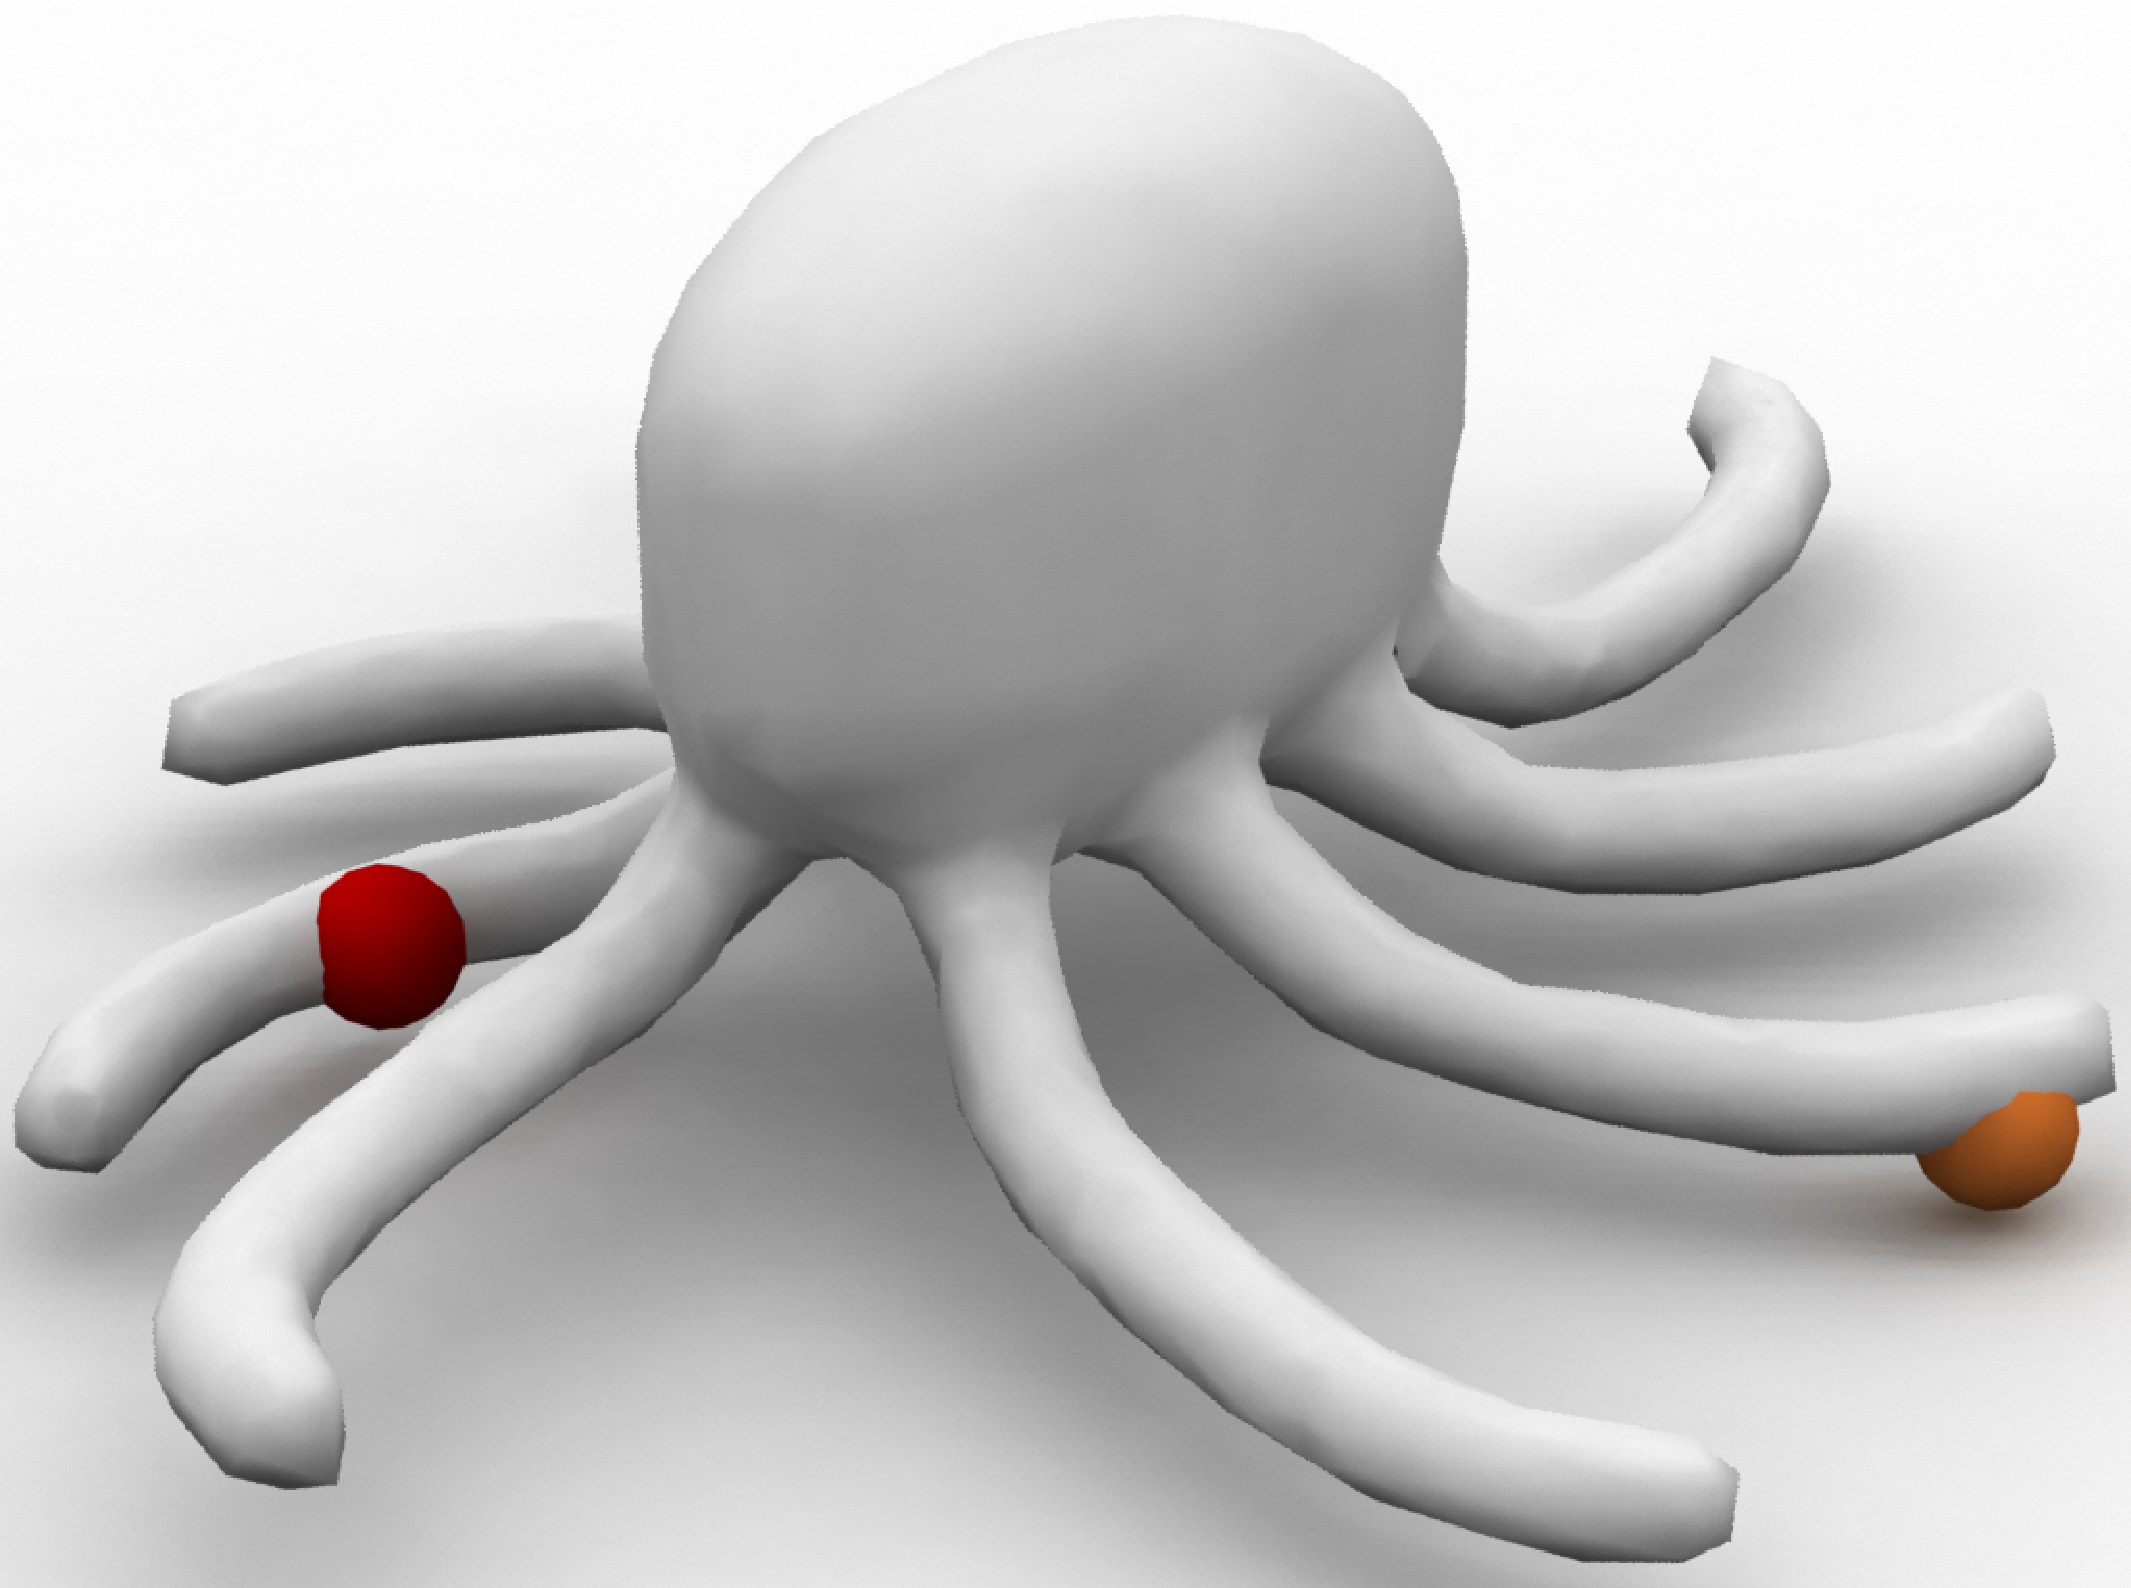
\includegraphics[height=.16\linewidth]{figures/regularization/source_octopus.pdf} &
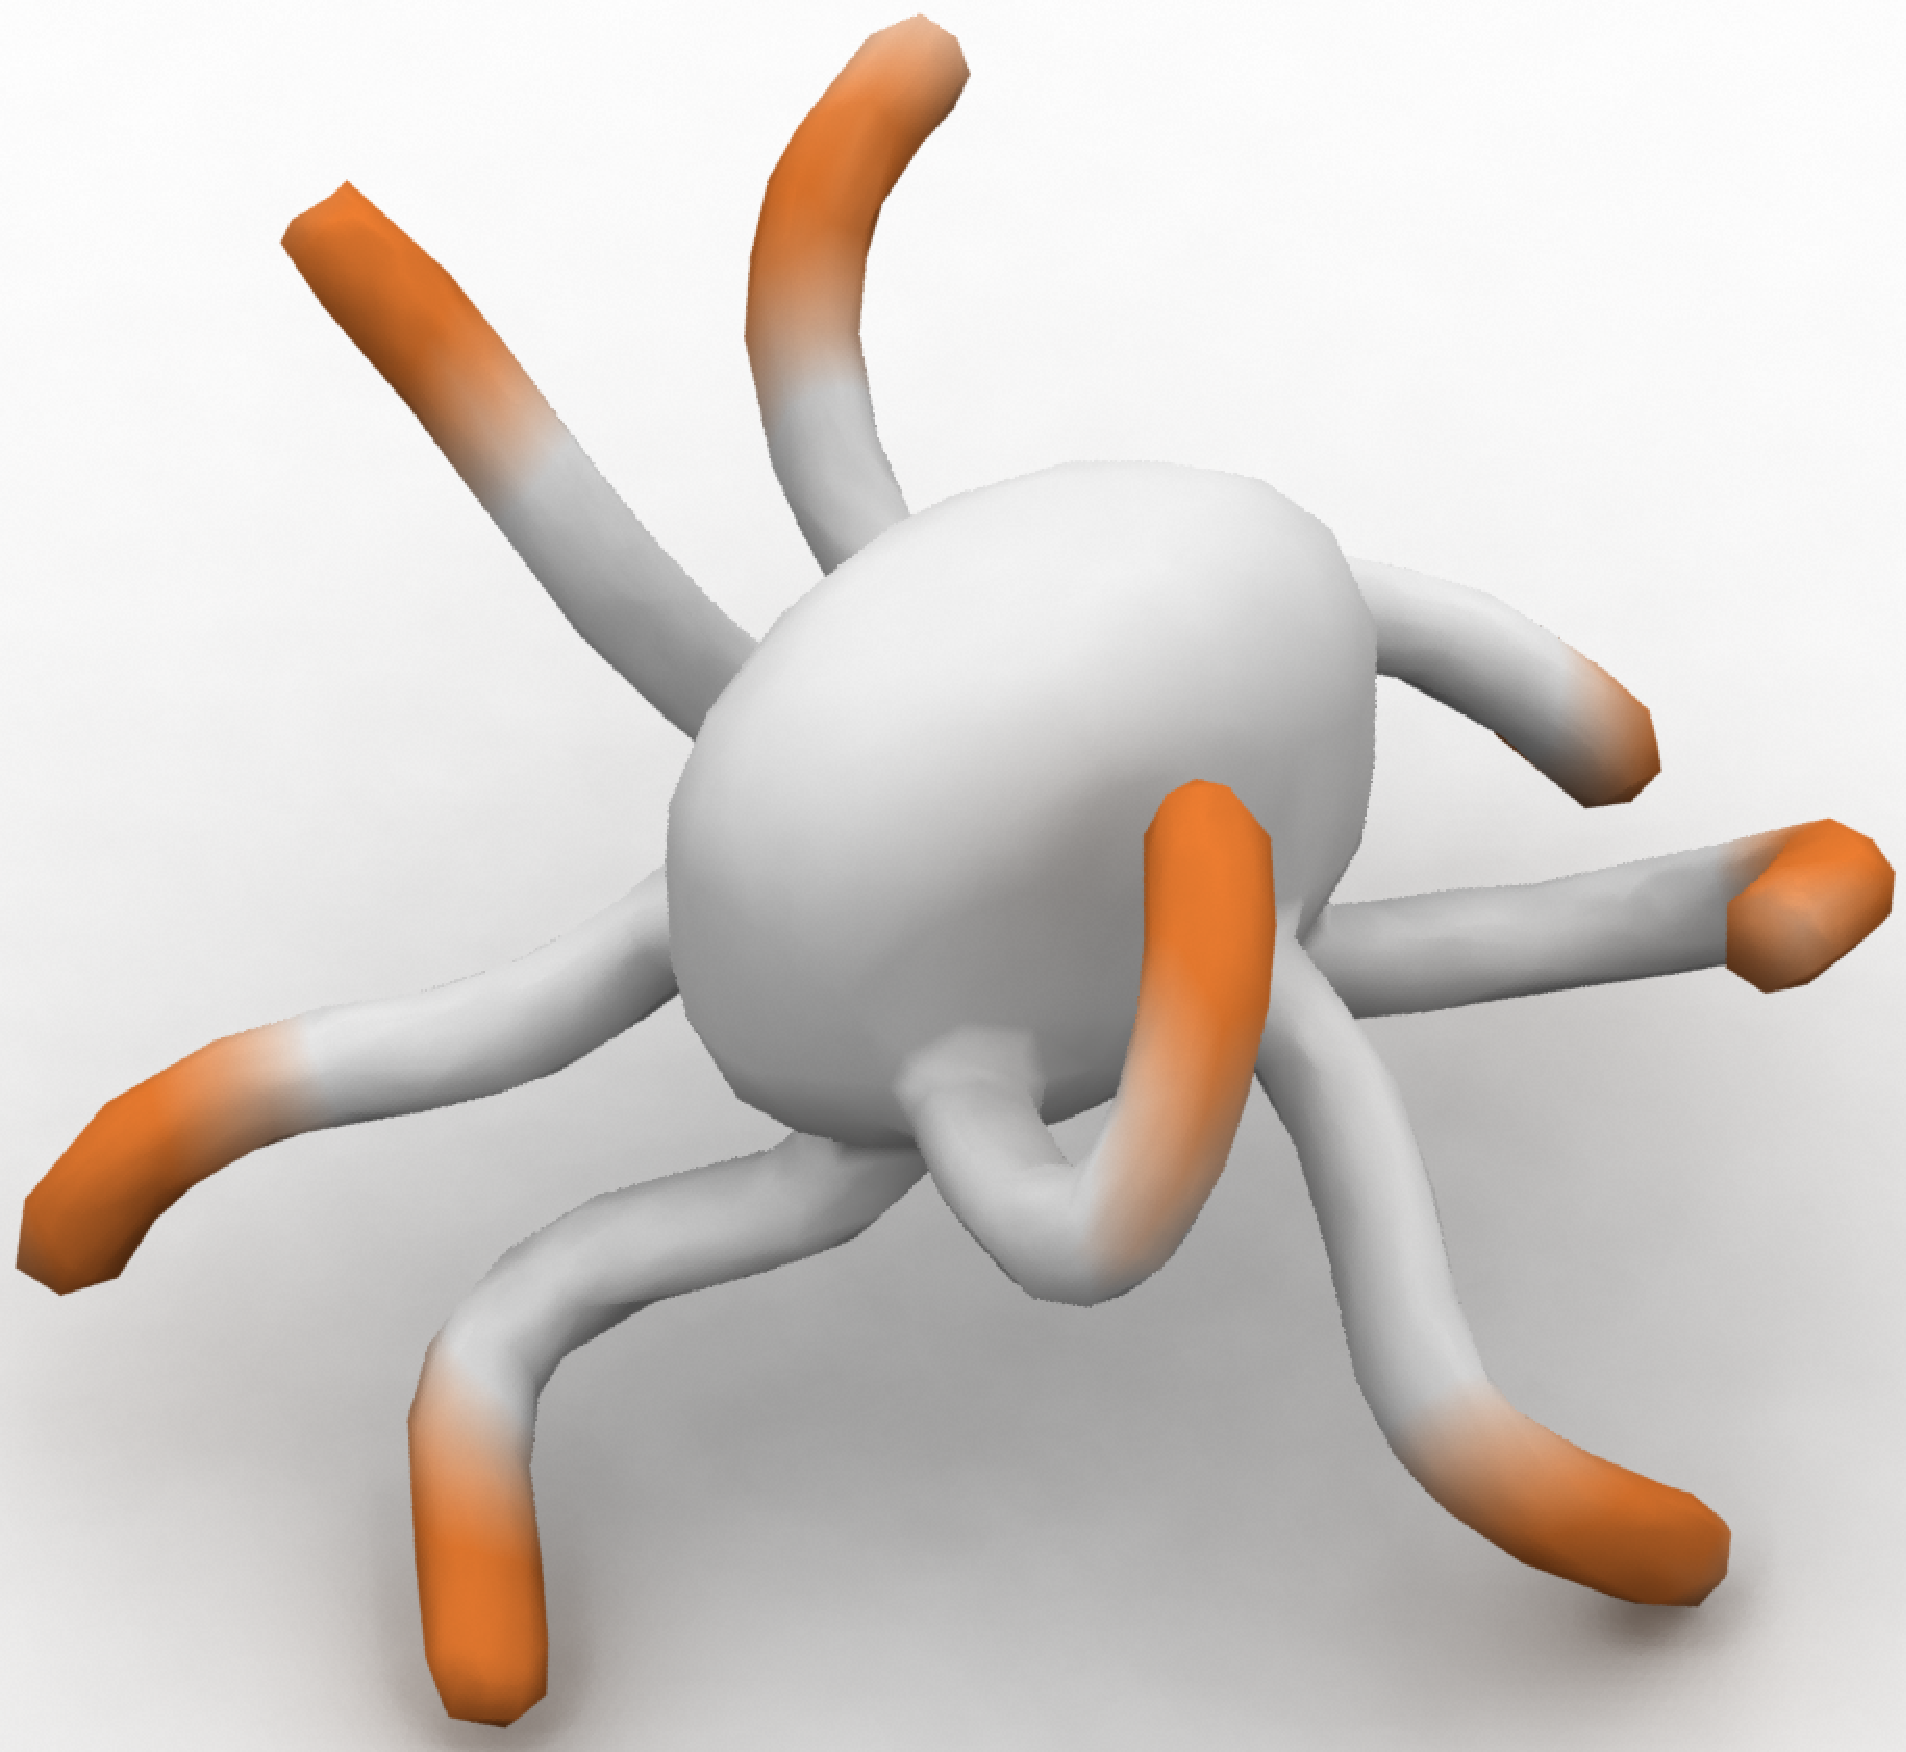
\includegraphics[height=.16\linewidth]{figures/regularization/target_octopus1_0.008.pdf}

\includegraphics[height=.16\linewidth]{figures/regularization/target_octopus2_0.008.pdf}
&
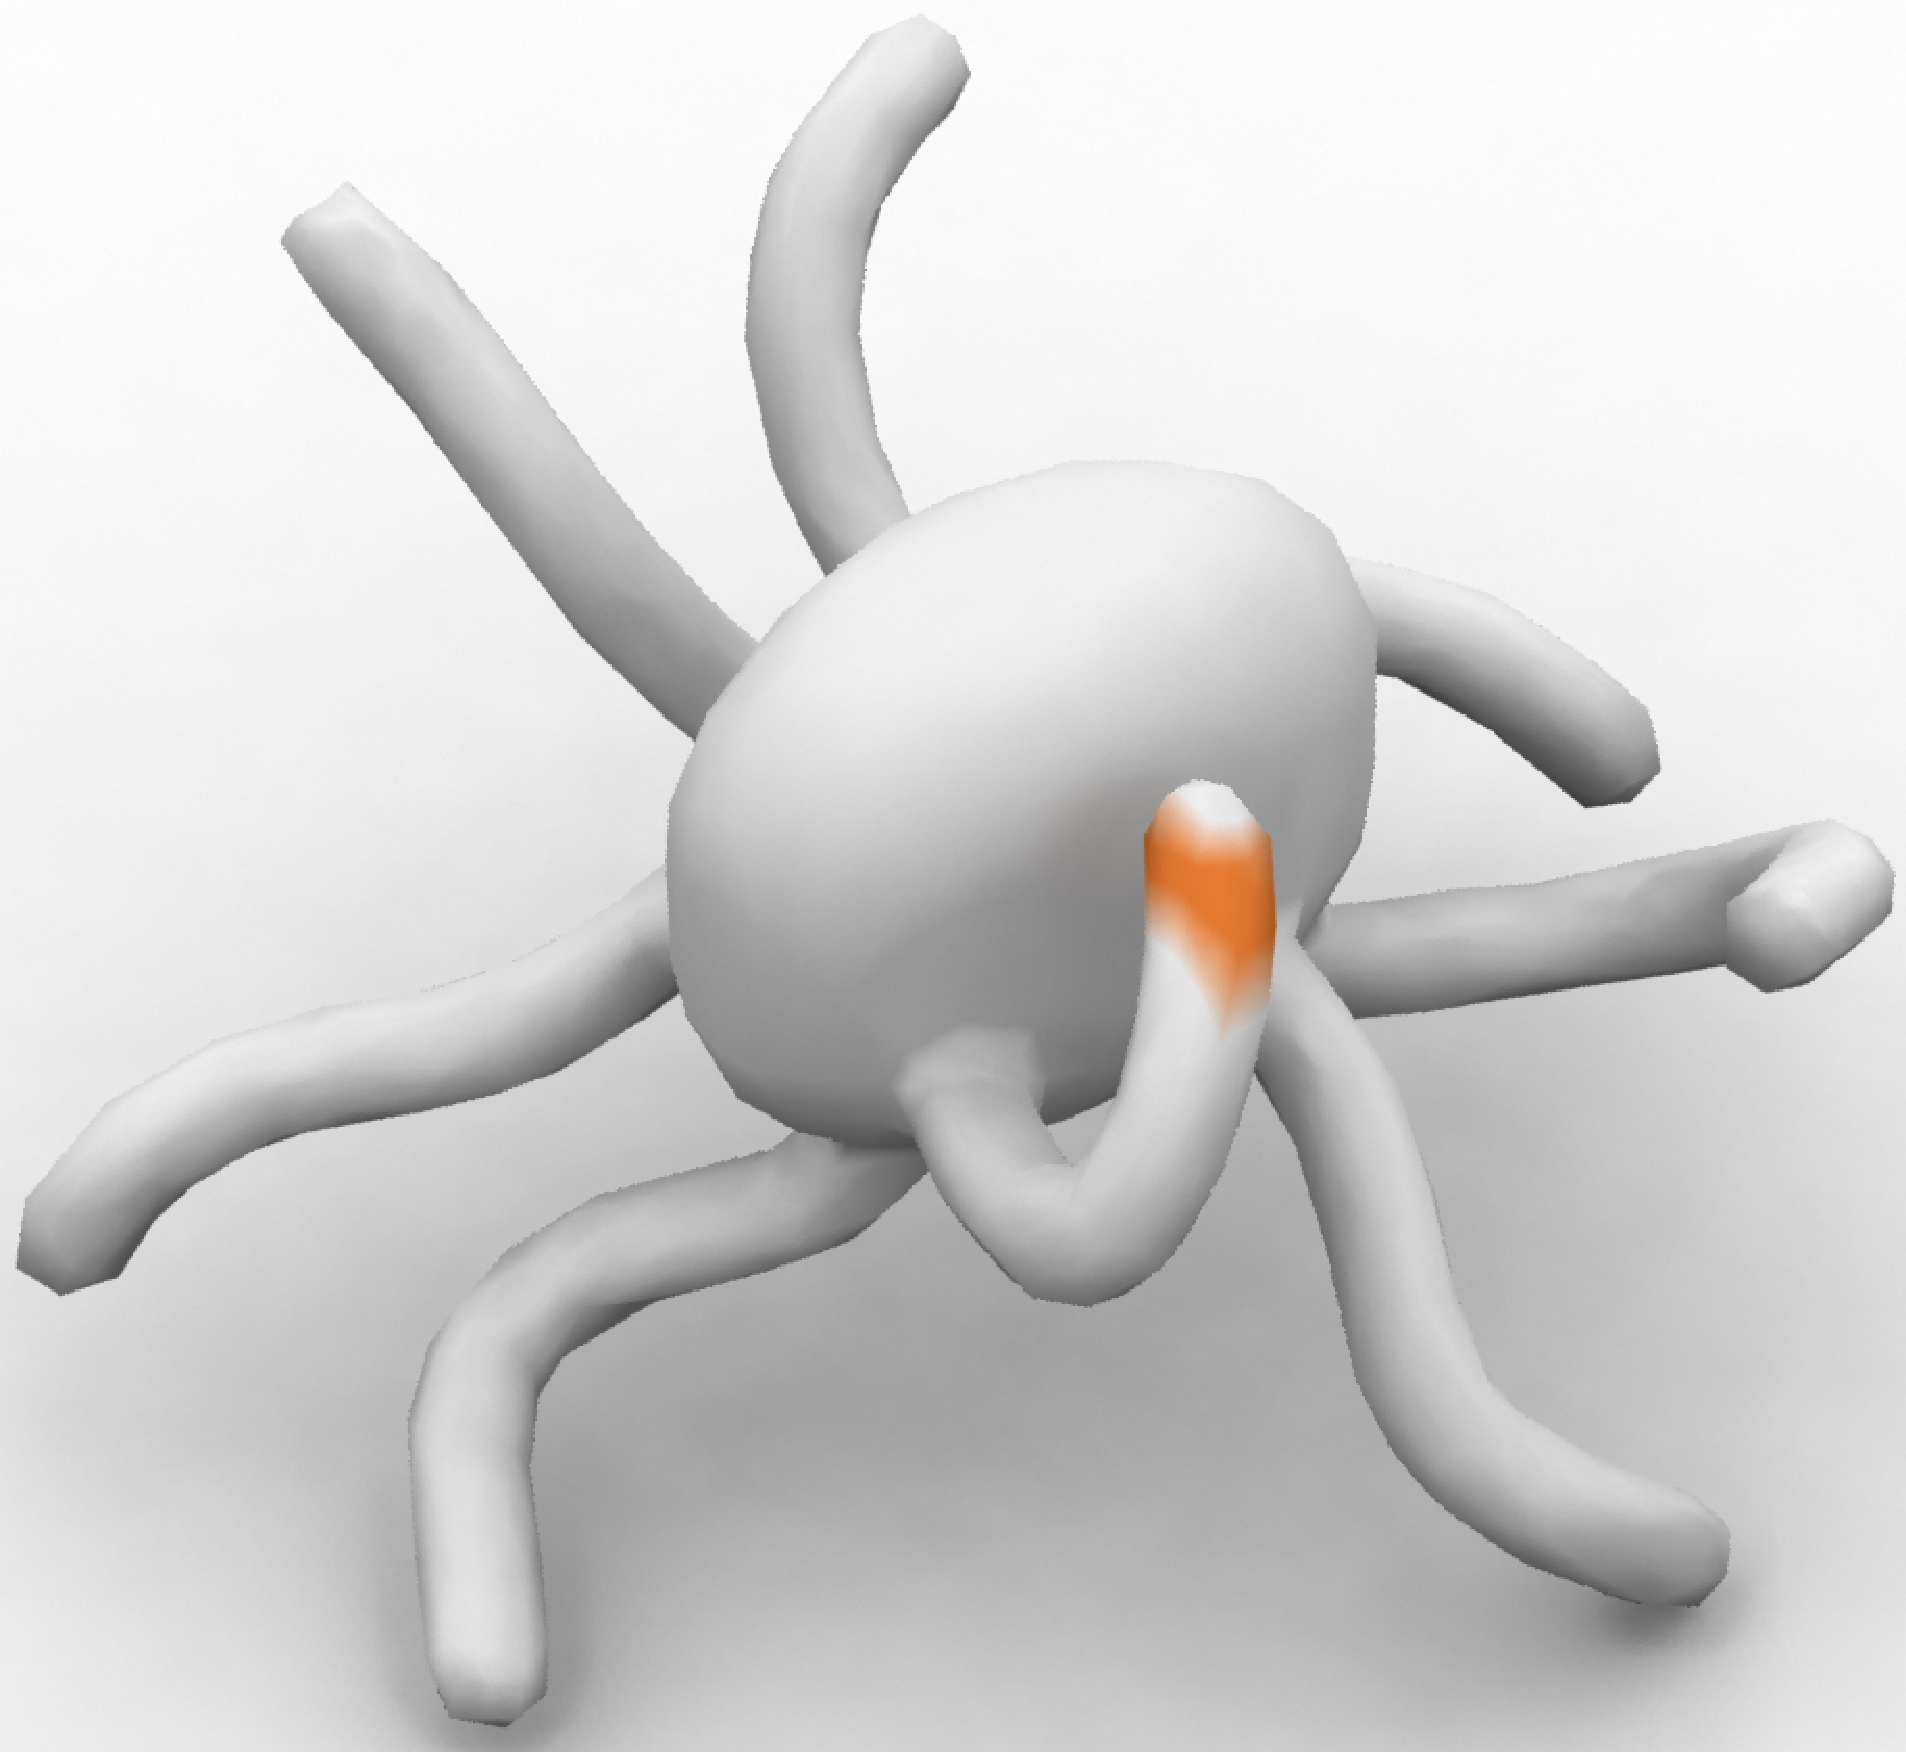
\includegraphics[height=.16\linewidth]{figures/regularization/target_octopus1_0.0007.pdf}
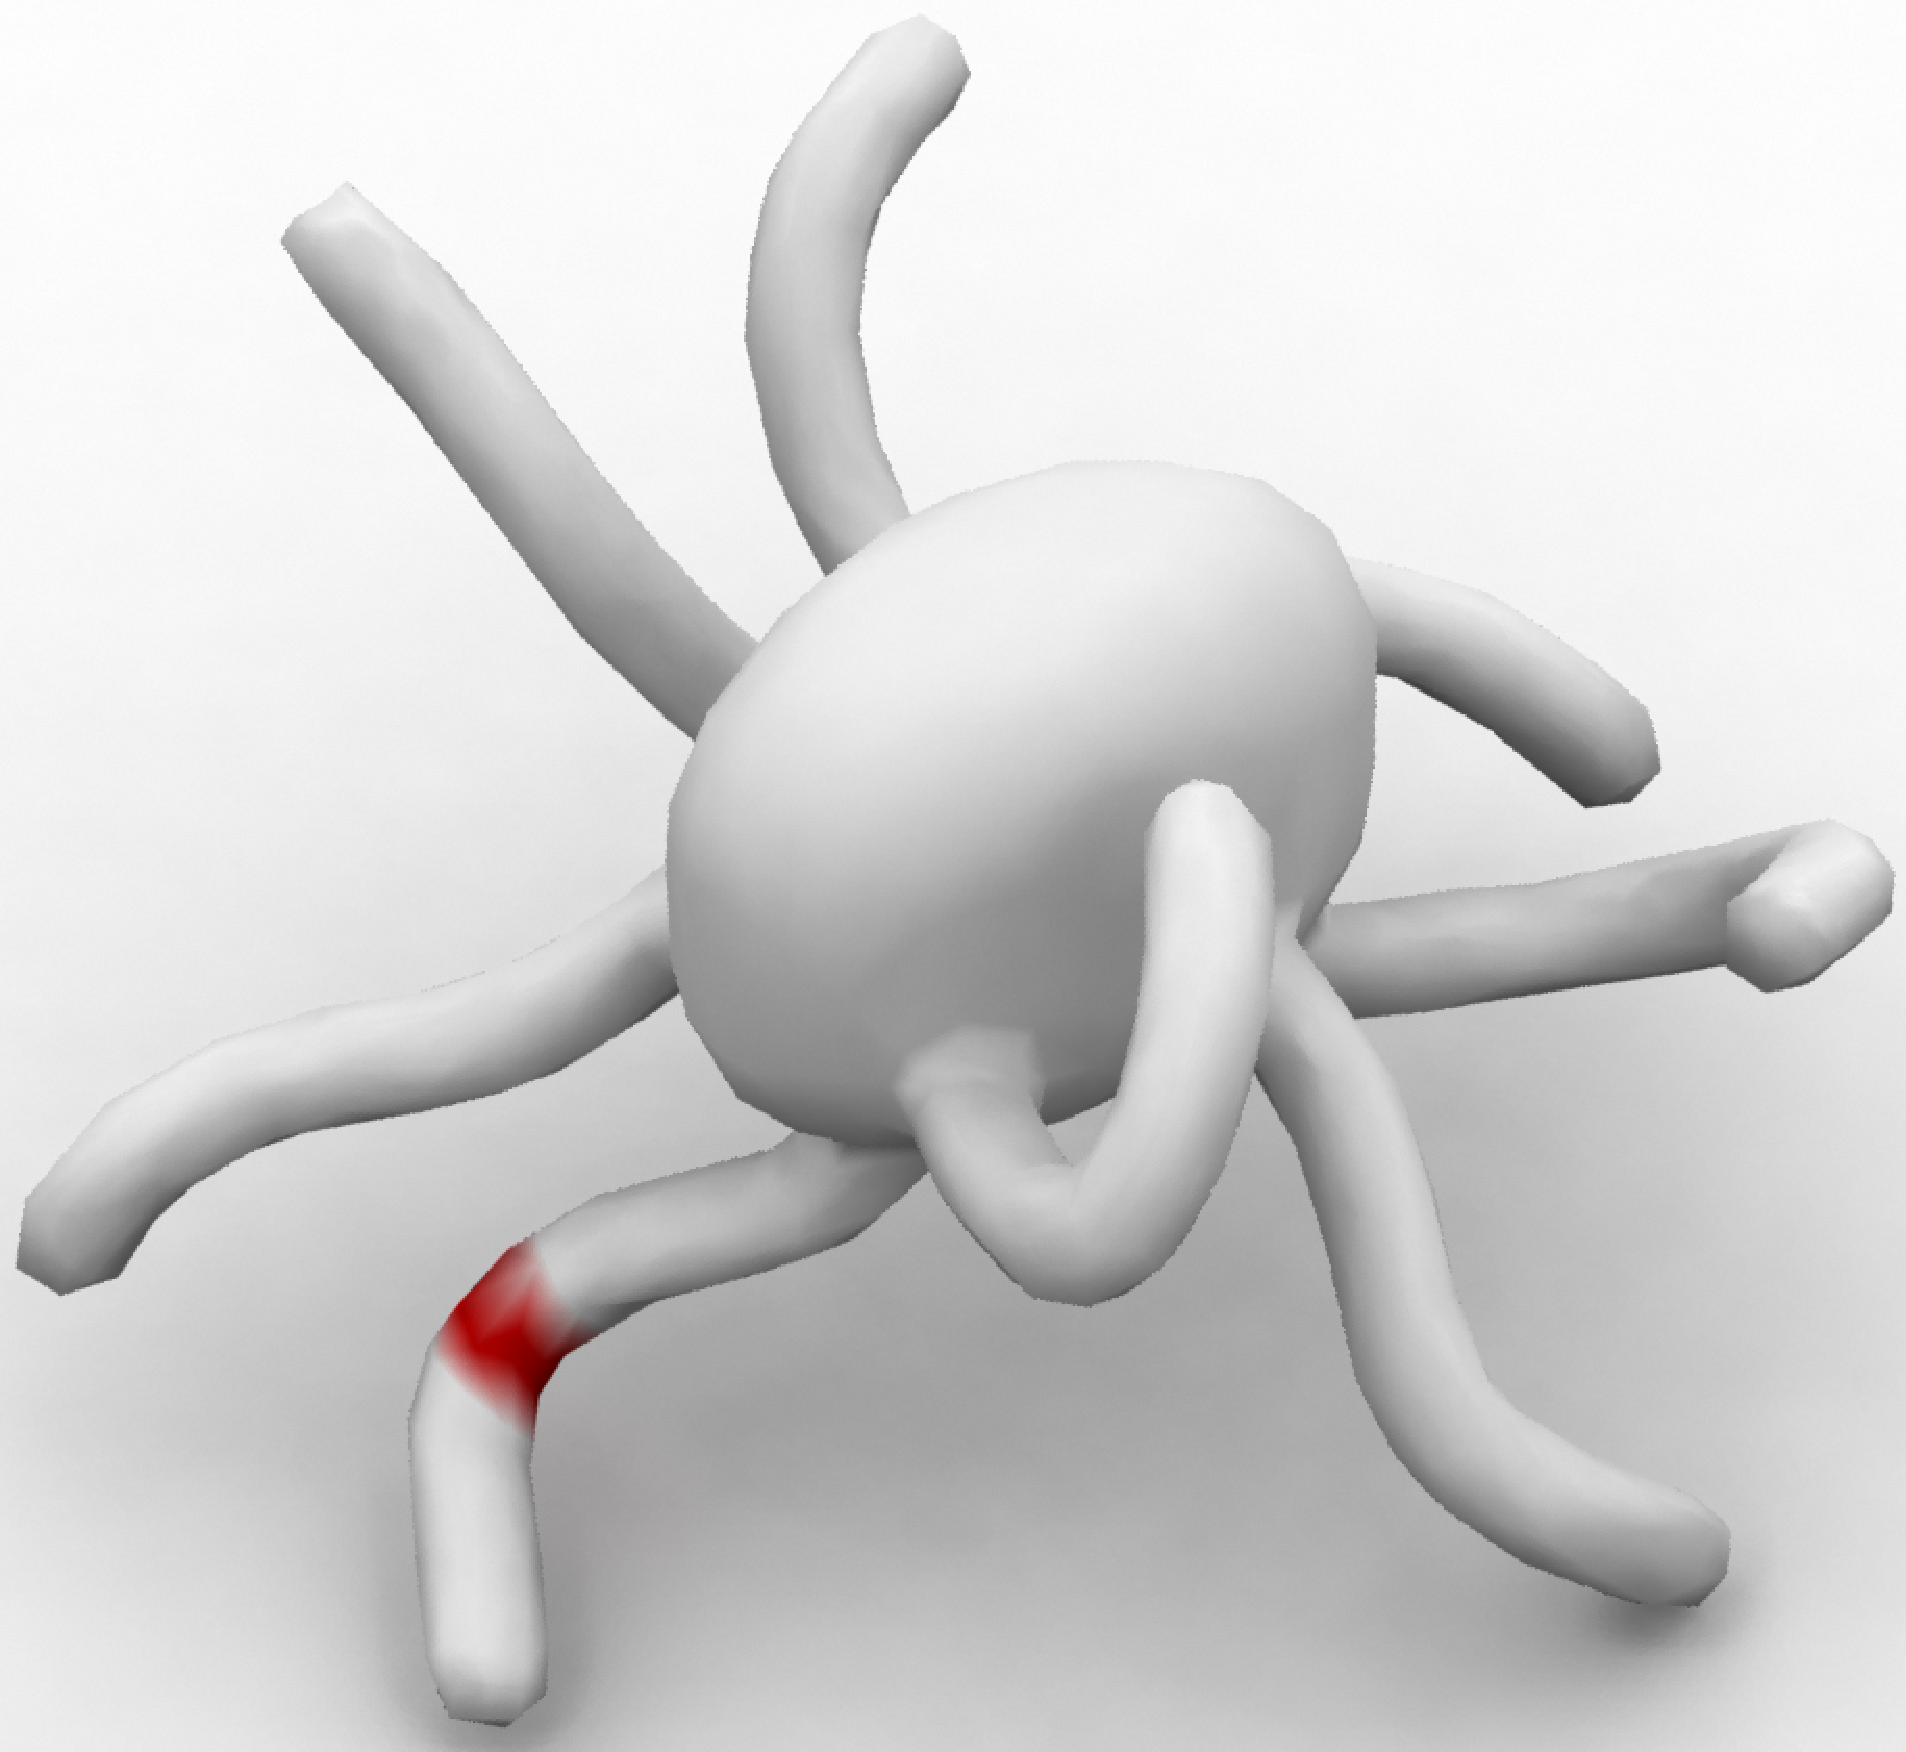
\includegraphics[height=.16\linewidth]{figures/regularization/target_octopus2_0.0007.pdf}
\\
Source surface
& Target surface ($\alpha=8\times10^{-3}$)
& Target surface ($\alpha=7\times10^{-4}$)
\end{tabular}
\caption{Effect of regularization parameter $\alpha$.  Colored points (left) are mapped to colored distributions (right).  As $\alpha$ decreases, the map sharpens; eventually, eight-way symmetry is broken in favor of a more bijective map matching tentacles based on asymmetries in their lengths.\vspace{-.2in}}\label{fig:reg}
\end{figure*}
Suppose we regularize the objective~\eqref{eq:discrete_optim_noreg} by adding $-\alpha H(\G)$ for some  $\alpha>0$.  As illustrated in Figure~\ref{fig:reg}, larger values of $\alpha$ increase the softness of $\G$, effectively smoothing the base GW objective function.  As $\alpha\rightarrow0$, optimal matchings $\G$ begin to resemble permutation matrices (see~\cite[eq.\ (10)]{quadrianto-2009}) and no longer superpose symmetric matches.

Now, define the \emph{KL-divergence} between $\G,\overline{\G}\in\R^{n_0\times n}_+$ as
$$\KL(\G|\overline{\G})\eqdef\sum_{ik} \bmu_{0i}\bmu_k \left[\left(\G\!_{ik} \ln\frac{\G\!_{ik}}{\overline{\G}\!_{ik}}\right)-\G\!_{ik}+\overline{\G}\!_{ik}\right]\!.$$
%\suv{Is the subsequent sentence needed? This particular KL divergence is also called the I-Divergence or simply generalized KL as you note.}%can't hurt to leave it there, right
This KL divergence contains an additional linear term from the one in~\cite{solomon-2015}, but since it only involves $\overline{\G}$ it is a constant in their objective.  This use of ``generalized'' KL (also called $I$-divergence) will figure into our method for joint domain analysis (\S\ref{sec:consistency}) and identifies KL divergence as a Bregman divergence~\cite{bregman-1967}.

\begin{algorithm}[t]
\fbox{\hspace{-.1in}\parbox{\columnwidth}{%
\begin{algorithmic}
\Function{Gromov-Wasserstein}{$\bmu_0,\D_0,\bmu,\D,\alpha,\eta$}
	\LineComment{Computes a local minimizer $\G$ of~\eqref{eq:reg_gw}}
	\algspace
	\Let{$\G$}{\Call{Ones}{$n_0\times n$}}
	\For{$i=1,2,3,\ldots$}
		\Let{$\K$}{$\exp(\D_0\diag{\bmu_0}\G\diag{\bmu}\D^\top/\alpha)$}
		\Let{$\G$}{\Call{Sinkhorn-Projection}{$\K^{\wedge \eta}\otimes \G^{\wedge (1-\eta)};\bmu_0,\bmu$}}
	\EndFor
%	\algspace
	\State\Return{$\G$}
\EndFunction
  \end{algorithmic}
}}
\algspace\\
\fbox{\hspace{-.1in}\parbox{\columnwidth}{%
\begin{algorithmic}
\Function{Sinkhorn-Projection}{$\K;\bmu_0,\bmu$}
	\LineComment{Finds $\G$ minimizing $\KL(\G|\K)$ subject to $\G\in\bM(\bmu_0,\bmu)$}
	\algspace
	\Let{$\v,\w$}{$\1$}%\Comment{Maintains $\G=\diag{\v}\G'\diag{\w}$}
	\For{$j= 1,2,3,\ldots$}
		\Let{$\v$}{$\1 \oslash \K(\w\otimes\bmu)$}
		\Let{$\w$}{$\1 \oslash \K^\top (\v\otimes\bmu_0)$}
	\EndFor
%	\algspace
	\State\Return{$\diag{\v}\K\diag{\w}$}
\EndFunction
  \end{algorithmic}
}}
\vspace{-3mm}
\caption{Iteration for finding regularized Gromov-Wasserstein distances.  $\otimes,\oslash$ denote elementwise multiplication and division.\vspace{-.2in}}\label{alg:gw}
\end{algorithm}

Finally, define
$$\f_\alpha(\G)\eqdef \exp(\D_0\diag{\bmu_0}\G\diag{\bmu}\D/\alpha).$$
After regularizing by adding $-\alpha H(\G)$ to the objective~\eqref{eq:discrete_optim_noreg}, an identical argument to the one in~\cite{benamou-2015} shows that we can recover $\G$ by solving the following minimization problem: % The resulting regularized version of~\eqref{eq:discrete_optim_noreg} can be written as
\begin{equation}\label{eq:reg_gw}
%\bGWa(\D_0,\D)\eqdef
\argmin_{\G\in\bM(\bmu_0,\bmu)} \alpha\KL(\G|\f_\alpha(\G)).
\end{equation}
The fact that $\G$ appears twice makes this objective nonconvex.  As derived in Appendix~\ref{appendix:convergence}, we compute $\G$ using KL-projected gradient descent:%\gabriel{maybe some more details would be welcome, it might not be obvious to everyone why this is a projected gradient. }
%\suv{What does gradient descent in the KL metric really mean? KL is no metric...}%changed to "kl-projected gradient descent"
\begin{equation}\label{eq:fixed_point_gw}
\boxed{\G^{(k\!+\!1)}\!\gets\!\argmin_{\G\in\bM}%(\bmu_0,\bmu)}
%
\KL\!\left(\!\G\!
\left|\!
\left[\f_\alpha(\G^{(k)})\right]^{\wedge\eta}\!\otimes\!\left[\G^{(k)}\right]^{\wedge(1-\eta)}\right.
\!\right)\!,}
\end{equation}
where $\otimes$ denotes elementwise (Hadamard) matrix multiplication.

Iteration~\eqref{eq:fixed_point_gw} is a convex program identical to the optimal transportation problems considered in~\cite{benamou-2015}; as derived in that paper, it can be optimized using iterative Sinkhorn projection.  The parameter $\eta\in(0,1]$ controls the \emph{inertia} of the iterative scheme; $\eta$ acts similarly to the ``learning rate'' parameter of gradient descent algorithms.  Pseudocode is provided in Algorithm~\ref{alg:gw}.  

\subsection{Convergence}\label{sec:convergence}

Convergence of~\eqref{eq:fixed_point_gw} as $k\rightarrow\infty$ is a subtle matter.  While existing work suggests monotonicity of the objective~\eqref{eq:reg_gw} under weak assumptions (see below), this does \emph{not} guarantee convergence of the iterates $\G^{(k)}\!$.  Given the dependence of our subsequent discussion on this algorithm as well as its appearance in many other contexts, we prove the following convergence result:
\begin{proposition}\label{prop:gw_convergence}
$\{\G^{(k)}\}_{k=0}^\infty$ converges to a critical point of~\eqref{eq:reg_gw} when $\eta<\nicefrac{c\alpha}{1+c\alpha}$, where $c\eqdef[\min_{ij}\bmu_{0i}\bmu_j]/\|\bmu_0\|^2\|\bmu\|^2\|\D_0\|\|\D\|$.
\end{proposition}
As $\alpha$ increases, the required bound loosens, reflecting the improved conditioning of the optimization problem.  We prove this result in the appendix by expressing it as an instance of a modern method for nonconvex optimization~\cite{bot-2015}.

From a practical standpoint, we halt \GWa iteration when the relative change in $\G$ or objective value is less than a fixed threshold ($10^{-7}$ in our experiments).

\paragraph*{Comparison to softassign.}  While we derived it for \GWa matching, iteration~\eqref{eq:fixed_point_gw} with $\eta=1$ is similar to the ``softassign'' algorithm in machine learning for quadratic assignment~\cite{gold-1996,rangarajan-1996}.  %, although this work only considers convex instances of the non-regularized quadratic correspondence problem and hence cannot deal with symmetric matching.
Rangarajan et al.~\shortcite{rangarajan-1997,rangarajan-1999} consider the convergence of softassign.  They mainly focus on monotonicity of the objective rather than convergence of the iterates.  More critically, their analysis assumes convexity; see, e.g., the conclusion of the proof of~\cite[Theorem 1]{rangarajan-1999}.  Such an assumption is unlikely to be valid for geometric problems with local and global symmetries.  Their analysis introduces convexity via a ``self-amplification term'' along the diagonal of the objective matrix, which modifies the optimization problem and obliterates the possibility of identifying symmetric ambiguity.

\subsection{Parameter Selection}

%\vova{Can we somehow guess an appropriate level of regularization?  Vova suggests showing that you can get away with low regularization when the shapes are isometric, and more is needed as you deviate from isometry.}

\begin{figure}\centering\pgfplotsset{scaled y ticks=false}
\begin{tikzpicture}
\begin{axis}[xlabel={\footnotesize $\alpha$},ylabel={\footnotesize Objective term},width=\columnwidth,height=.5\columnwidth,
xlabel near ticks,
ylabel near ticks,
line cap = round,
line join = round,
xlabel shift = -.04in,
ylabel shift = -.08in,
xmin = 0.0007,
xmax = .1,
ymin = 0,
yticklabel style={
        /pgf/number format/fixed,
        /pgf/number format/precision=3
},xmode=log,%ymode=log,
scaled y ticks=false,legend cell align=left]%,legend pos = south west]
\addplot[mark=none,color=blue,thick] table[x index=0,y index=1,col sep=comma,mark=none] {figures/alpha/alphatest.txt};\addlegendentry{\footnotesize $\langle \G,\bL(\G)\rangle$};
\addplot[mark=none,color=purple,thick] table[x index=0,y index=2,col sep=comma,mark=none] {figures/alpha/alphatest.txt};\addlegendentry{\footnotesize $-H(\G)$};
\end{axis}
\end{tikzpicture}
\vspace{-.15in}
\caption{Dependence of objective terms on regularizer $\alpha$ for the experiment in Figure~\protect\ref{fig:reg}.\vspace{-.15in}}\label{fig:regularizer}
\end{figure}

%\gabriel{So the conclusion here seems to be that large $\alpha$ is not so helpful :( This somehow contradict the conclusion of the article, I found.}\justin{how so?  large alpha makes for fast convergence and maps that superpose symmetries, both good things for fuzzy mapping!  added a few sentences}

Figure~\ref{fig:regularizer} illustrates the trade-off between the two objective terms for the experiments in Figure~\ref{fig:reg} as a function of $\alpha$.  As $\alpha$ increases, so does the GW objective~\eqref{eq:GW2} while negative entropy decreases.  A phase transition in the GW objective indicates a change in the nature of the map, in this case from mapping individual tentacles to superposing all tentacle targets.  This example illustrates a more general pattern:  large choices of $\alpha$ lead to higher-entropy correspondence matrices that still contain meaningful match information, while lower $\alpha$'s make for sharper map matrices that express a single coherent matching.  When $\alpha$ is small but there exist multiple symmetric maps, they can be extracted using the method in \S\ref{sec:symmetry}.

Our algorithm converges faster with a warm start, and hence we can generate plots like the one in Figure~\ref{fig:regularizer} efficiently by incrementally adjusting $\alpha$ and updating $\G$.  User-guided selection of $\alpha$ can be guided using this plot to find significant changes in the map as it depends on regularization.



% Doesn't seem to work
%\section{Partial Matching}
%
%If we assume that every point in $\source$ has some match in $\target$ but not necessarily the reverse, then we should not optimize in the space of measure couplings $\M(\mu_0,\mu)$ but rather in a simpler space of measures satisfying only the first constraint $\gamma(S_0\times \target)=\mu_0(S_0)\,\forall S_0\subseteq\source.$
%
%Discretely, this suggests a larger space of partial couplings:
%$$\bP(\bmu_0,\bmu)\eqdef\{\G\in\R_+^{n_0\times n} : \G\bmu=\1\}.$$
%Iterative optimization of our regularized objective with this new set of constraints is essentially the same as before~\eqref{eq:fixed_point_gw}:
%\begin{equation}
%\boxed{
%\G^{(k\!+\!1)}\!\gets\!
%\argmin_{\G\in\bP}\!\,\KL\!\left(
%\!\G\!\left|\!\,
%\exp\!\left(-\frac{\eta}{\alpha}\bL(\G^{(\!k\!)})\!\right)
%\!\otimes\!
%\left[\!\G^{(\!k\!)}\!\right]\!^{\!\wedge\!(1\!-\!\eta)}
%\right.
%\right)\!
%}
%\end{equation}
%In this case, the KL projection is even simpler than the Sinkhorn projection needed in \S\ref{sec:entropic_reg}; rather than requiring iterative normalization, the rows of the kernel are simply scaled to integrate to one.
%
%Taking the partial matching philosophy to the extreme, we could remove all marginal constraints on $\G$ and instead require that it represent a general distribution over $\source\times\target$.   In discrete language, this variation corresponds to constraining only $\bmu_0^\top\G\bmu=1$ and $\G\geq0$.  KL projection onto this set maps $\K\mapsto\K/(\bmu_0^\top\K\bmu)$. 
%
% This final relaxation is dangerous in the continuous case and even discretely when the entropic regularizer is not introduced.  In the extreme, $\G$ could have just a single nonzero entry matching a single point on the source and target.  The entropic regularizer, however, counteracts this concentrated match by encouraging $\G$ to have a wider distribution of nonzero entries.  Both algorithms for partial matching are made explicit in Algorithm~\ref{alg:partial_gw}.
%
%
%\begin{algorithm}[t]
%\fbox{\hspace{-.1in}\parbox{\columnwidth}{%
%\begin{algorithmic}
%\Function{Partial-Source-GW}{$\bmu_0,\D_0,\bmu,\D,\alpha$}
%	\LineComment{Gromov-Wasserstein with only prescribed row sums}
%	\algspace
%	\Let{$\G$}{\Call{Ones}{$n_0\times n$}}
%	\For{$i=1,2,3,\ldots$}
%		\Let{$\K$}{
%$
%\left\{
%\begin{array}{r@{}l}
%\exp[\frac{1}{\alpha}
%(\D_0&\diag{\bmu_0}\G\diag{\bmu}\D^\top\\
%&-\frac{1}{2}\1\bmu_0^\top\G\diag{\bmu}\D^{\wedge2})]
%\end{array}\right.
%$}
%		\Let{$\K$}{$\K^{\wedge \eta}\otimes\G^{\wedge(1-\eta)}$}
%		\Let{$\G$}{$\K\oslash (\K\bmu\1^\top)$}
%	\EndFor
%	\algspace
%	\State\Return{$\G$}
%\EndFunction
%  \end{algorithmic}
%}}
%\algspace\\
%\fbox{\hspace{-.1in}\parbox{\columnwidth}{%
%\begin{algorithmic}
%\Function{Partial-to-Partial-GW}{$\bmu_0,\D_0,\bmu,\D,\alpha$}
%	\LineComment{Gromov-Wasserstein without prescribed marginals}
%	\algspace
%	\Let{$\G$}{\Call{Ones}{$n_0\times n$}}
%	\For{$i=1,2,3,\ldots$}
%		\Let{$\K$}{
%$
%\left\{
%\begin{array}{r@{}l}
%\exp[\frac{1}{\alpha}
%(\D_0&\diag{\bmu_0}\G\diag{\bmu}\D^\top\\
%&-\frac{1}{2}\1\bmu_0^\top\G\diag{\bmu}\D^{\wedge2}\\
%&-\frac{1}{2}\D_0^{\wedge2}\diag{\bmu_0}\G\bmu\1^\top
%)]
%\end{array}\right.
%$}
%		\Let{$\K$}{$\K^{\wedge \eta}\otimes\G^{\wedge(1-\eta)}$}
%		\Let{$\G$}{$\K/(\bmu_0^\top \K\bmu)$}
%	\EndFor
%	\algspace
%	\State\Return{$\G$}
%\EndFunction
%  \end{algorithmic}
%}}
%\caption{Algorithms for partial matching that optimize the Gromov-Wasserstein objective.}\label{alg:partial_gw}
%\end{algorithm}


%%% Local Variables:
%%% mode: latex
%%% TeX-master: "../gw"
%%% End:
